\begin{figure}[t]
  \centering
  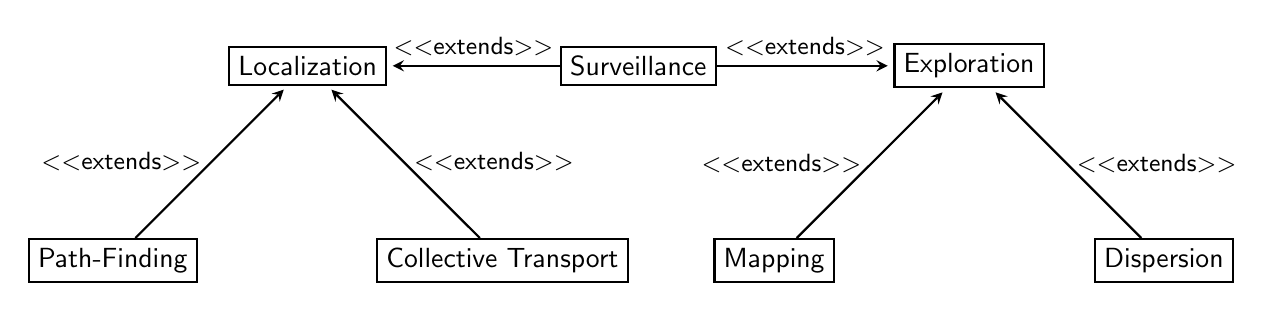
\begin{tikzpicture}[->,>=stealth,shorten >=2pt,auto,node distance=3.5cm,
    thick,main node/.style={fill=white,draw,font=\sffamily}]
    \node[main node] (1) {Localization};
    \node[main node] (2) [below left of=1] {Path-Finding};
    \node[main node] (3) [below right of=1] {Collective Transport};
    \node[main node] (4) [right of=1,node distance=4.2cm] {Surveillance};
    \node[main node] (5) [right of=4,node distance=4.2cm] {Exploration};
    \node[main node] (7) [below left of=5] {Mapping};
    \node[main node] (6) [below right of=5] {Dispersion};

    \path[every node/.style={font=\sffamily\small}]
      (2) edge node [left] {$<<$extends$>>$} (1)
      (3) edge [right] node[right] {$<<$extends$>>$} (1)
      (4) edge [right] node[above] {$<<$extends$>>$} (1)
      (4) edge [right] node[above] {$<<$extends$>>$} (5)
      (6) edge [right] node[right] {$<<$extends$>>$} (5)
      (7) edge [right] node[left] {$<<$extends$>>$} (5);
  \end{tikzpicture}
  \caption{Technique Hierarchy Overview} \label{fig:TechniquesMindMap}
\end{figure}
